\documentclass[12pt,a4paper]{article}
\usepackage[utf8]{inputenc}
\usepackage{polski}
\usepackage[polish]{babel}
\usepackage{graphicx}
\usepackage{hyperref}
\usepackage[margin=2.5cm]{geometry}
\usepackage{listings}
\usepackage{xcolor}
\usepackage{amsmath}
\usepackage{enumitem}
\usepackage{tikz}
\usepackage{float}
\usepackage{svg}

% Konfiguracja listingów kodu
\definecolor{codegreen}{rgb}{0,0.6,0}
\definecolor{codegray}{rgb}{0.5,0.5,0.5}
\definecolor{codepurple}{rgb}{0.58,0,0.82}
\definecolor{backcolour}{rgb}{0.95,0.95,0.95}

\lstdefinestyle{mystyle}{
    backgroundcolor=\color{backcolour},   
    commentstyle=\color{codegreen},
    keywordstyle=\color{blue},
    stringstyle=\color{codepurple},
    basicstyle=\ttfamily\scriptsize,
    breakatwhitespace=false,         
    breaklines=true,                 
    captionpos=b,                    
    keepspaces=true,                 
    numbersep=5pt,                  
    showspaces=false,                
    showstringspaces=false,
    showtabs=false,                  
    tabsize=2
}

\lstset{style=mystyle}



\begin{document}
\begin{titlepage}
\begin{center}
\large
{\noindent Collegium Witelona Uczelnia Państwowa w Legnicy}\\
{\noindent Wydział Nauk Technicznych i Ekonomicznych}\\
{\noindent Kierunek: Informatyka}\\[2cm]

\includegraphics[width=5cm]{godlo.jpg}\\[2cm]
{\large\textbf{Projekt z przedmiotu Projektowanie systemów baz danych}}\\[0.3cm]
{\noindent Temat: System zarządzania wypożyczalnią samochodów.}\\[3cm]
{\large\textbf{Autorzy}}\\
Mateusz Bogacz-Drewniak, nr. indeksu: 44491\\
Paweł Kruk, nr. indeksu: 43845\\[0.3cm]
Grupa: 1(2)\\[3cm]
\end{center}

\begin{flushright}
\begin{tabular}{l}
Prowadzący przedmiot\\
mgr inż. Roman Hojniak
\end{tabular}
\end{flushright}

\vfill
\begin{center}
{\noindent Legnica, 2025}
\end{center}
\end{titlepage}

\tableofcontents

\newpage

\section{Koncepcja}

\subsection{Cel projektu bazy danych}

Celem projektu jest stworzenie systemu zarządzania wypożyczalnią samochodów, który umożliwi efektywne zarządzanie flotą pojazdów, obsługę klientów oraz monitorowanie procesu wypożyczeń. System ma na celu usprawnienie procesów biznesowych związanych z wypożyczaniem pojazdów, umożliwienie użytkownikom przeglądania dostępnych samochodów, dokonywania rezerwacji oraz zarządzania swoimi wypożyczeniami.

Główne cele systemu:
\begin{itemize}
    \item Zapewnienie platformy do zarządzania flotą pojazdów
    \item Udostępnienie klientom możliwości przeglądania i wypożyczania samochodów
    \item Zapewnienie efektywnego systemu rezerwacji i kontroli dostępności pojazdów
    \item Monitorowanie wypożyczeń i kontrola terminów zwrotu
    \item Zarządzanie klientami, w tym możliwość blokowania nieuczciwych użytkowników
    \item Śledzenie i rejestrowanie zmian dokonywanych w systemie dla celów audytu i kontroli
\end{itemize}

\subsection{Opis dziedziny przedmiotowej}

Wypożyczalnia samochodów to firma usługowa, która udostępnia pojazdy klientom na określony czas za odpowiednią opłatą. Proces wypożyczenia obejmuje kilka kluczowych etapów:

\begin{enumerate}
    \item \textbf{Rejestracja klienta} - nowy użytkownik musi zarejestrować się w systemie podając swoje dane osobowe i adresowe
    \item \textbf{Przeglądanie dostępnych pojazdów} - użytkownik przegląda dostępne samochody wraz z ich specyfikacjami
    \item \textbf{Proces wypożyczenia} - wybór samochodu, określenie dat wypożyczenia, potwierdzenie
    \item \textbf{Zarządzanie wypożyczeniem} - monitorowanie terminów, przedłużanie, zwrot
\end{enumerate}

\newpage

System obsługuje dwa główne typy użytkowników: klientów (osoby wypożyczające) oraz administratorów (pracowników wypożyczalni). Administratorzy mają dostęp do szerszych funkcjonalności, takich jak zarządzanie flotą, dodawanie nowych pojazdów, przeglądanie wszystkich wypożyczeń oraz zarządzanie czarną listą klientów.

Kluczowymi elementami dziedziny są:
\begin{itemize}
    \item \textbf{Samochody} - pojazdy dostępne do wypożyczenia wraz z ich parametrami
    \item \textbf{Klienci} - osoby korzystające z usług wypożyczalni
    \item \textbf{Wypożyczenia} - rekordy dotyczące wypożyczonych pojazdów, dat i osób wypożyczających
    \item \textbf{Administratorzy} - osoby zarządzające systemem
    \item \textbf{Czarna lista} - lista klientów z ograniczonym dostępem do usług
\end{itemize}

% Miejsce na diagram procesu wypożyczenia samochodu
\begin{figure}[H]
    \centering
    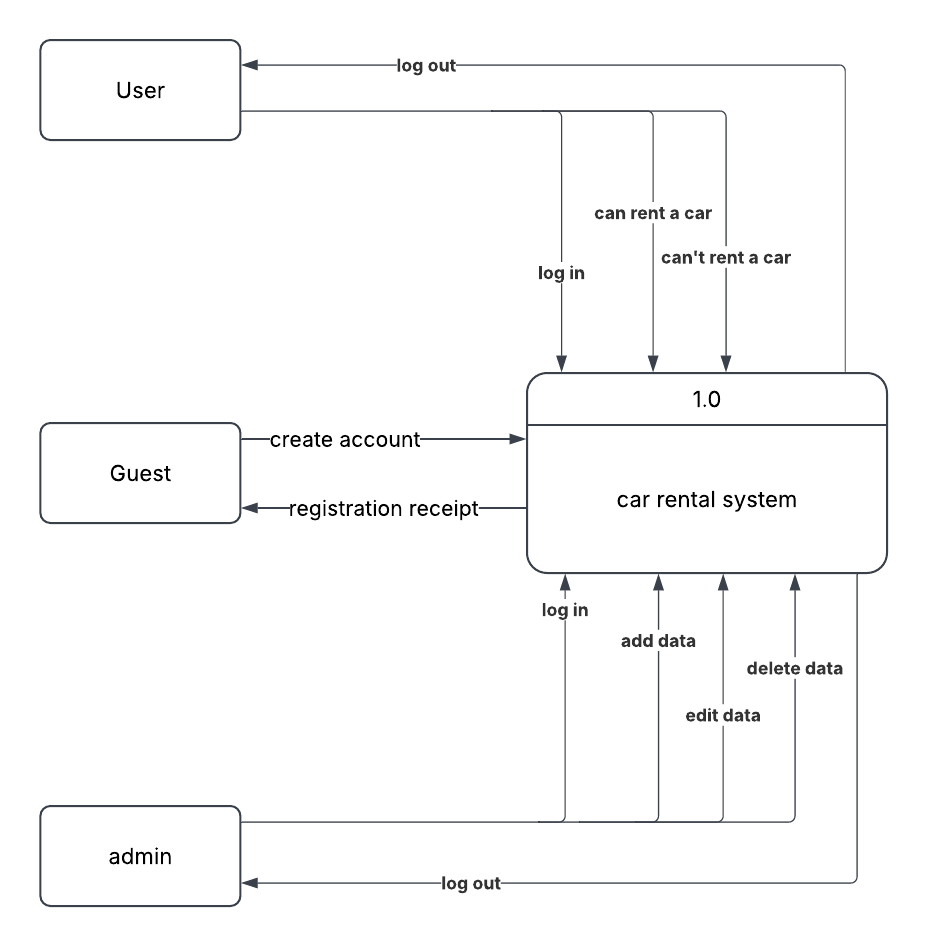
\includegraphics[width=0.8\textwidth]{dfd_lvl_0.png}
    \caption{Proces wypożyczenia samochodu}
    \label{fig:proces-wypozyczenia}
\end{figure}

\newpage

\subsection{Założenia wstępne}

Projekt systemu został oparty na następujących założeniach:

\begin{enumerate}
    \item \textbf{Platforma technologiczna}:
    \begin{itemize}
        \item Framework Django (Python)
        \item Relacyjna baza danych (PostgreSQL)
        \item Interfejs webowy (HTML, CSS, JavaScript)
        \item Konteneryzacja (Docker)
    \end{itemize}
    
    \item \textbf{Struktura danych}:
    \begin{itemize}
        \item System przechowuje dane o samochodach, klientach, administratorach, wypożyczeniach i blokadach
        \item Każdy samochód posiada swoją specyfikację i zdjęcia
        \item Klienci posiadają dane osobowe oraz adresowe
        \item Wypożyczenia zawierają informacje o datach, użytkowniku i wypożyczonym pojeździe
    \end{itemize}
    
    \item \textbf{Funkcjonalność}:
    \begin{itemize}
        \item Dwupoziomowy system uprawnień (administrator/użytkownik)
        \item Mechanizm autentykacji i autoryzacji
        \item Zarządzanie dostępnością pojazdów
        \item System blokowania nieuczciwych klientów
        \item Zarządzanie zdjęciami pojazdów
    \end{itemize}
    
    \item \textbf{Interfejs}:
    \begin{itemize}
        \item Responsywny interfejs użytkownika
        \item Oddzielne panele dla klientów i administratorów
        \item Przejrzysty katalog pojazdów z filtrowaniem
        \item Intuicyjny system rezerwacji
    \end{itemize}
\end{enumerate}

\newpage

\section{Specyfikacja wymagań systemu}

\subsection{Użytkownicy systemu oraz ich role}

System obsługuje trzy główne typy użytkowników:

\subsubsection{Niezalogowani użytkownicy}
\textbf{Uprawnienia}:
\begin{itemize}
    \item Przeglądanie strony głównej
    \item Rejestracja w systemie
    \item Logowanie do systemu
\end{itemize}

\subsubsection{Zalogowani klienci (Użytkownicy)}
\textbf{Uprawnienia}:
\begin{itemize}
    \item Przeglądanie dostępnych samochodów
    \item Wyświetlanie szczegółów pojazdów
    \item Wypożyczanie samochodów
    \item Przeglądanie własnych wypożyczeń
    \item Edycja własnych danych osobowych
\end{itemize}

\textbf{Ograniczenia}:
\begin{itemize}
    \item Brak dostępu do panelu administracyjnego
    \item Brak możliwości modyfikacji danych samochodów
    \item Brak możliwości wypożyczenia jeśli użytkownik jest na czarnej liście
\end{itemize}

\subsubsection{Administratorzy}
\textbf{Uprawnienia}:
\begin{itemize}
    \item Zarządzanie flotą samochodów (dodawanie, edycja, usuwanie)
    \item Zarządzanie danymi pojazdów (w tym zdjęcia)
    \item Zarządzanie wypożyczeniami
    \item Zarządzanie użytkownikami
    \item Dodawanie i usuwanie użytkowników z czarnej listy
    \item Zarządzanie innymi administratorami
    \item Zarządzanie adresami
\end{itemize}

\begin{figure}[H]
    \centering
    \includesvg[angle=90,width=1.4\textwidth]{dfd_lvl_1.svg}
    \caption{Diagram przypadków użycia systemu}
    \label{fig:use-case-diagram}
\end{figure}

\newpage

\subsection{Wymagania funkcjonalne}

\subsubsection{Moduł autentykacji}
\begin{itemize}
    \item F1.1: System umożliwia rejestrację nowych użytkowników
    \item F1.2: System zapewnia logowanie dla użytkowników i administratorów
    \item F1.3: System umożliwia wylogowanie z systemu
    \item F1.4: System weryfikuje uprawnienia użytkowników do dostępu do funkcji
\end{itemize}

\subsubsection{Moduł zarządzania użytkownikami}
\begin{itemize}
    \item F2.1: System umożliwia administratorowi przeglądanie wszystkich użytkowników
    \item F2.2: System umożliwia administratorowi dodawanie nowych użytkowników
    \item F2.3: System umożliwia administratorowi edycję danych użytkowników
    \item F2.4: System umożliwia administratorowi usuwanie użytkowników
    \item F2.5: System umożliwia dodawanie użytkowników do czarnej listy
    \item F2.6: System umożliwia usuwanie użytkowników z czarnej listy
    \item F2.7: System umożliwia administratorowi zarządzanie adresami użytkowników
\end{itemize}

\subsubsection{Moduł zarządzania samochodami}
\begin{itemize}
    \item F3.1: System umożliwia administratorowi dodawanie nowych samochodów
    \item F3.2: System umożliwia administratorowi edycję danych samochodów
    \item F3.3: System umożliwia administratorowi usuwanie samochodów
    \item F3.4: System umożliwia administratorowi zarządzanie zdjęciami samochodów
    \item F3.5: System wyświetla szczegóły wybranego samochodu
    \item F3.6: System umożliwia administratorowi zarządzanie kolejnością zdjęć samochodów
\end{itemize}

\subsubsection{Moduł wypożyczeń}
\begin{itemize}
    \item F4.1: System umożliwia klientom wypożyczanie dostępnych samochodów
    \item F4.2: System weryfikuje dostępność samochodu przed wypożyczeniem
    \item F4.3: System weryfikuje czy klient nie jest na czarnej liście
    \item F4.4: System umożliwia administratorowi przeglądanie wszystkich wypożyczeń
    \item F4.5: System umożliwia administratorowi dodawanie, edycję i usuwanie wypożyczeń
    \item F4.6: System wyświetla historię wypożyczeń dla każdego samochodu
\end{itemize}

\subsubsection{Moduł historii zmian}
\begin{itemize}
    \item F5.1: System rejestruje wszystkie operacje wykonywane na danych (INSERT, UPDATE, DELETE)
    \item F5.2: System umożliwia administratorowi przeglądanie historii zmian
    \item F5.3: System umożliwia filtrowanie historii zmian według różnych kryteriów
    \item F5.4: System umożliwia eksport historii zmian do formatu CSV
\end{itemize}

\subsection{Wymagania niefunkcjonalne}

\subsubsection{Wymagania dotyczące użyteczności}
\begin{itemize}
    \item NF1.1: System posiada intuicyjny interfejs użytkownika
    \item NF1.2: Interfejs systemu jest responsywny i dostosowany do różnych urządzeń
    \item NF1.3: System informuje użytkowników o statusie wykonywanych operacji (komunikaty sukcesu, błędu)
    \item NF1.4: System obsługuje standardowe formaty zdjęć (JPG, PNG, GIF, BMP)
\end{itemize}

\subsubsection{Wymagania dotyczące wydajności}
\begin{itemize}
    \item NF2.1: System odpowiada na zapytania użytkownika w czasie krótszym niż 2 sekundy
    \item NF2.2: System obsługuje jednoczesne wypożyczanie tego samego samochodu przez wielu użytkowników
    \item NF2.3: System efektywnie zarządza zasobami serwera (pamięć, CPU)
\end{itemize}

\subsubsection{Wymagania dotyczące bezpieczeństwa}
\begin{itemize}
    \item NF3.1: Hasła użytkowników są przechowywane w formie zahaszowanej
    \item NF3.2: System zabezpiecza przed nieautoryzowanym dostępem do panelu administracyjnego
    \item NF3.3: System zabezpiecza dane przed atakami typu SQL Injection i Cross-Site Scripting
    \item NF3.4: System wymaga uwierzytelnienia do dostępu do funkcji klienta i administratora
\end{itemize}

\subsubsection{Wymagania dotyczące niezawodności}
\begin{itemize}
    \item NF4.1: System jest dostępny 24/7 z wyjątkiem zaplanowanych przerw konserwacyjnych
    \item NF4.2: System obsługuje błędy w sposób elegancki, dostarczając użytkownikowi informacje o problemie
    \item NF4.3: System posiada procedury tworzenia kopii zapasowych danych
\end{itemize}

\newpage
\section{Model danych}

\subsection{Schemat bazy danych}

% Miejsce na diagram ERD
\begin{figure}[H]
    \centering
    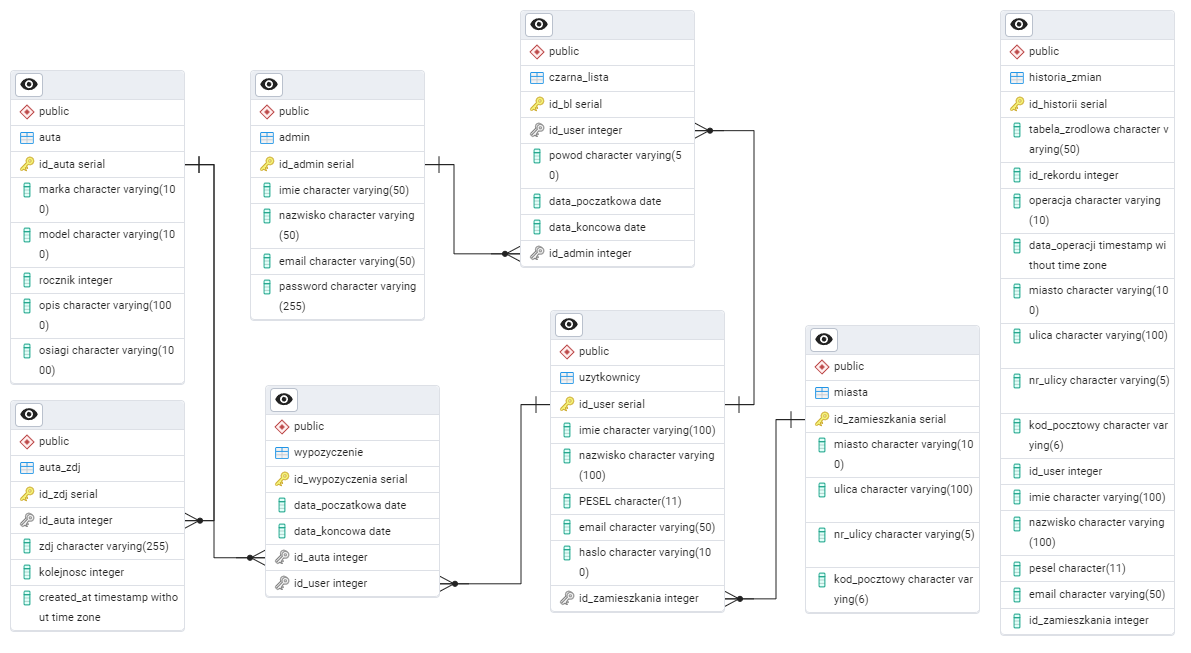
\includegraphics[width=1\textwidth]{erd.png}
    \caption{Diagram relacji encji (ERD) bazy danych}
    \label{fig:erd-diagram}
\end{figure}

Relacje między tabelami:
\begin{enumerate}
    \item Użytkownik (Uzytkownicy) ma jeden adres (Miasta) - relacja jeden do wielu
    \item Samochód (Auta) może mieć wiele zdjęć (AutaZdj) - relacja jeden do wielu
    \item Samochód (Auta) może być w wielu wypożyczeniach (Wypozyczenie) - relacja jeden do wielu
    \item Użytkownik (Uzytkownicy) może mieć wiele wypożyczeń (Wypozyczenie) - relacja jeden do wielu
    \item Użytkownik (Uzytkownicy) może być na czarnej liście (CzarnaLista) - relacja jeden do wielu
    \item Administrator (Admin) może dodać wielu użytkowników do czarnej listy (CzarnaLista) - relacja jeden do wielu
\end{enumerate}

\newpage

\subsection{Opis poszczególnych encji}

\subsubsection{Auta}
Tabela przechowująca informacje o samochodach dostępnych w wypożyczalni.

\begin{table}[H]
\centering
\begin{tabular}{|l|l|p{7cm}|}
\hline
\textbf{Pole} & \textbf{Typ} & \textbf{Opis} \\
\hline
id\_auta & AutoField (PK) & Unikalny identyfikator samochodu \\
\hline
marka & CharField(100) & Marka samochodu \\
\hline
model & CharField(100) & Model samochodu \\
\hline
rocznik & IntegerField & Rok produkcji \\
\hline
opis & CharField(1000) & Opis samochodu \\
\hline
osiagi & CharField(1000) & Osiągi samochodu \\
\hline
\end{tabular}
\caption{Struktura tabeli Auta}
\end{table}

\subsubsection{AutaZdj}
Tabela przechowująca zdjęcia samochodów.

\begin{table}[H]
\centering
\begin{tabular}{|l|l|p{7cm}|}
\hline
\textbf{Pole} & \textbf{Typ} & \textbf{Opis} \\
\hline
id\_zdj & AutoField (PK) & Unikalny identyfikator zdjęcia \\
\hline
id\_auta & ForeignKey & Powiązanie z samochodem \\
\hline
zdj & CharField(255) & Ścieżka do pliku zdjęcia \\
\hline
kolejnosc & IntegerField & Kolejność wyświetlania zdjęcia \\
\hline
created\_at & DateTimeField & Data dodania zdjęcia \\
\hline
\end{tabular}
\caption{Struktura tabeli AutaZdj}
\end{table}

\subsubsection{Miasta}
Tabela przechowująca adresy użytkowników.

\begin{table}[H]
\centering
\begin{tabular}{|l|l|p{7cm}|}
\hline
\textbf{Pole} & \textbf{Typ} & \textbf{Opis} \\
\hline
id\_zamieszkania & AutoField (PK) & Unikalny identyfikator adresu \\
\hline
miasto & CharField(100) & Nazwa miasta \\
\hline
ulica & CharField(100) & Nazwa ulicy \\
\hline
nr\_ulicy & CharField(5) & Numer budynku \\
\hline
kod\_pocztowy & CharField(6) & Kod pocztowy (format: XX-XXX) \\
\hline
\end{tabular}
\caption{Struktura tabeli Miasta}
\end{table}

\newpage

\subsubsection{Użytkownicy}
Tabela przechowująca dane użytkowników systemu.

\begin{table}[H]
\centering
\begin{tabular}{|l|l|p{7cm}|}
\hline
\textbf{Pole} & \textbf{Typ} & \textbf{Opis} \\
\hline
id\_user & AutoField (PK) & Unikalny identyfikator użytkownika \\
\hline
imie & CharField(100) & Imię użytkownika \\
\hline
nazwisko & CharField(100) & Nazwisko użytkownika \\
\hline
pesel & CharField(11) & Numer PESEL \\
\hline
email & CharField(50) & Adres email (używany do logowania) \\
\hline
haslo & CharField(100) & Zahaszowane hasło użytkownika \\
\hline
id\_zamieszkania & ForeignKey & Powiązanie z adresem zamieszkania \\
\hline
\end{tabular}
\caption{Struktura tabeli Użytkownicy}
\end{table}

\subsubsection{Admin}
Tabela przechowująca dane administratorów systemu.

\begin{table}[H]
\centering
\begin{tabular}{|l|l|p{7cm}|}
\hline
\textbf{Pole} & \textbf{Typ} & \textbf{Opis} \\
\hline
id\_admin & AutoField (PK) & Unikalny identyfikator administratora \\
\hline
imie & CharField(50) & Imię administratora \\
\hline
nazwisko & CharField(50) & Nazwisko administratora \\
\hline
email & CharField(50) & Adres email (używany do logowania) \\
\hline
haslo & CharField(255) & Zahaszowane hasło administratora \\
\hline
\end{tabular}
\caption{Struktura tabeli Admin}
\end{table}

\subsubsection{Wypozyczenie}
Tabela przechowująca informacje o wypożyczeniach.

\begin{table}[H]
\centering
\begin{tabular}{|l|l|p{7cm}|}
\hline
\textbf{Pole} & \textbf{Typ} & \textbf{Opis} \\
\hline
id\_wypozyczenia & AutoField (PK) & Unikalny identyfikator wypożyczenia \\
\hline
data\_poczatkowa & DateField & Data rozpoczęcia wypożyczenia \\
\hline
data\_koncowa & DateField & Data zakończenia wypożyczenia \\
\hline
id\_auta & ForeignKey & Powiązanie z wypożyczanym samochodem \\
\hline
id\_user & ForeignKey & Powiązanie z użytkownikiem wypożyczającym \\
\hline
\end{tabular}
\caption{Struktura tabeli Wypozyczenie}
\end{table}

\newpage

\subsubsection{CzarnaLista}
Tabela przechowująca informacje o użytkownikach na czarnej liście.

\begin{table}[H]
\centering
\begin{tabular}{|l|l|p{7cm}|}
\hline
\textbf{Pole} & \textbf{Typ} & \textbf{Opis} \\
\hline
id\_bl & AutoField (PK) & Unikalny identyfikator wpisu \\
\hline
id\_user & ForeignKey & Powiązanie z użytkownikiem \\
\hline
powod & CharField(50) & Powód dodania do czarnej listy \\
\hline
data\_poczatkowa & DateField & Data rozpoczęcia blokady \\
\hline
data\_koncowa & DateField & Data zakończenia blokady \\
\hline
id\_admin & ForeignKey & Administrator, który dodał wpis \\
\hline
\end{tabular}
\caption{Struktura tabeli CzarnaLista}
\end{table}

\subsubsection{HistoriaZmian}
Tabela przechowująca historię operacji wykonywanych na danych w systemie.

\begin{table}[H]
\centering
\begin{tabular}{|l|l|p{7cm}|}
\hline
\textbf{Pole} & \textbf{Typ} & \textbf{Opis} \\
\hline
id\_historii & AutoField (PK) & Unikalny identyfikator wpisu historii \\
\hline
tabela\_zrodlowa & CharField(50) & Nazwa tabeli, której dotyczy operacja \\
\hline
id\_rekordu & IntegerField & ID rekordu, którego dotyczy operacja \\
\hline
operacja & CharField(10) & Rodzaj operacji (INSERT, UPDATE, DELETE) \\
\hline
data\_operacji & DateTimeField & Data i czas wykonania operacji \\
\hline
miasto & CharField(100) & Miasto (jeśli dotyczy) \\
\hline
ulica & CharField(100) & Ulica (jeśli dotyczy) \\
\hline
nr\_ulicy & CharField(5) & Numer ulicy (jeśli dotyczy) \\
\hline
kod\_pocztowy & CharField(6) & Kod pocztowy (jeśli dotyczy) \\
\hline
id\_user & IntegerField & ID użytkownika (jeśli dotyczy) \\
\hline
imie & CharField(100) & Imię (jeśli dotyczy) \\
\hline
nazwisko & CharField(100) & Nazwisko (jeśli dotyczy) \\
\hline
pesel & CharField(11) & PESEL (jeśli dotyczy) \\
\hline
email & CharField(50) & Email (jeśli dotyczy) \\
\hline
id\_zamieszkania & IntegerField & ID zamieszkania (jeśli dotyczy) \\
\hline
\end{tabular}
\caption{Struktura tabeli HistoriaZmian}
\end{table}

\newpage

\subsection{Model MVC}

Aplikacja została zaimplementowana zgodnie z architekturą Model-View-Controller (MVC), która w Django jest nazywana często Model-Template-View (MTV). Poniżej przedstawiono podział komponentów aplikacji według tego wzorca:

\subsubsection{Model (Models)}
Modele reprezentują strukturę danych i logikę biznesową aplikacji:
\begin{itemize}
    \item \textbf{models.py} - zawiera definicje wszystkich klas modeli (Auta, AutaZdj, Miasta, Uzytkownicy, Admin, Wypozyczenie, CzarnaLista), które odpowiadają tabelom w bazie danych.
    \item \textbf{repositories/} - katalog zawierający klasy repozytoriów, które zapewniają dostęp do danych:
    \begin{itemize}
        \item \textbf{admin\_repository.py} - operacje na danych administratorów
        \item \textbf{blacklist\_repository.py} - operacje na danych czarnej listy
        \item \textbf{car\_repository.py} - operacje na danych samochodów i ich zdjęć
        \item \textbf{rental\_repository.py} - operacje na danych wypożyczeń
        \item \textbf{user\_repository.py} - operacje na danych użytkowników i adresów
        \item \textbf{change\_history\_repository.py} - operacje na danych historii zmian
    \end{itemize}
\end{itemize}

\subsubsection{Widok (Template)}
Szablony definiują sposób prezentacji danych użytkownikowi:
\begin{itemize}
    \item \textbf{templates/} - katalog zawierający wszystkie szablony HTML aplikacji:
    \begin{itemize}
        \item Strony główne: index.html, login.html, register.html
        \item Panel użytkownika: user\_dashboard.html, car\_detail.html, rent\_car.html, user\_ban\_info.html
        \item Panel administracyjny: admin\_dashboard.html, admin\_car\_view.html, admin\_car\_photos.html, admin\_address\_view.html, admin\_rent\_view.html, admin\_admin\_view.html, admin\_user\_view.html, admin\_blacklist\_view.html
        \item Komponenty wspólne: includes/navbar.html, includes/navbar1.html, includes/navbar2.html, includes/navbar3.html, includes/admin\_sidebar.html, includes/footer.html, includes/head.html
        \item Strony błędów: 400.html, 404.html, 500.html, error.html
    \end{itemize}
\end{itemize}

\newpage

\subsubsection{Kontroler (View / Controller)}
Kontrolery obsługują interakcje użytkownika i zarządzają przepływem danych:
\begin{itemize}
    \item \textbf{views.py} - zawiera funkcje widoków, które obsługują żądania HTTP i zwracają odpowiedzi
    \item \textbf{services/} - katalog zawierający klasy serwisów, które implementują logikę biznesową:
    \begin{itemize}
        \item \textbf{admin\_service.py} - logika biznesowa związana z administratorami
        \item \textbf{blacklist\_service.py} - logika biznesowa związana z czarną listą
        \item \textbf{car\_service.py} - logika biznesowa związana z samochodami
        \item \textbf{rental\_service.py} - logika biznesowa związana z wypożyczeniami
        \item \textbf{user\_service.py} - logika biznesowa związana z użytkownikami
        \item \textbf{change\_history\_service.py} - logika biznesowa związana z historią zmian
    \end{itemize}
    \item \textbf{forms.py} - zawiera definicje formularzy wykorzystywanych w aplikacji
    \item \textbf{urls.py} - definiuje mapowanie URL do funkcji widoków
\end{itemize}

% Miejsce na diagram MVC/MTV
\begin{figure}[H]
    \centering
    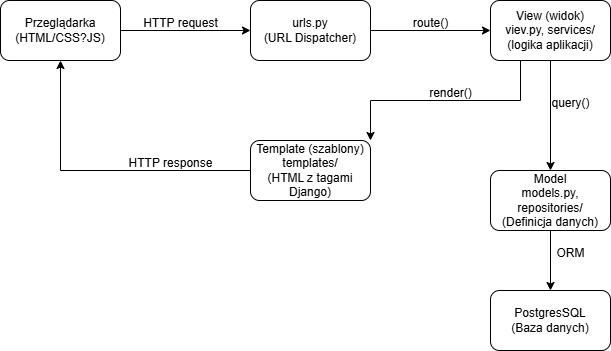
\includegraphics[width=1\textwidth]{diagram_mvc.png}
    \caption{Architektura Model-Template-View (MTV) aplikacji Django}
    \label{fig:mtv-architecture}
\end{figure}

\newpage

\section{Interfejs Użytkownika}

\subsection{Opis GUI}

System wykorzystuje interfejs webowy oparty na frameworku Bootstrap, co zapewnia responsywność i spójny wygląd na różnych urządzeniach. Interfejs podzielony jest na dwie główne części: panel użytkownika i panel administracyjny.

\subsubsection{Panel publiczny}
Dostępny dla niezalogowanych użytkowników:

\begin{enumerate}
    \item \textbf{Strona główna (index.html)}
    \begin{itemize}
        \item Prezentuje podstawowe informacje o wypożyczalni
        \item Zawiera przyciski do logowania i rejestracji
        \item Menu nawigacyjne z opcjami: Home, Login, Rejestracja
    \end{itemize}
    
    \item \textbf{Strona logowania (login.html)}
    \begin{itemize}
        \item Formularz logowania z polami: email, hasło
        \item Przekierowanie do odpowiedniego panelu (administratora lub użytkownika) po zalogowaniu
        \item Obsługa komunikatów błędów (np. nieprawidłowe dane logowania)
    \end{itemize}
    
    \item \textbf{Strona rejestracji (register.html)}
    \begin{itemize}
        \item Formularz rejestracji z sekcjami:
        \begin{itemize}
            \item Dane osobowe (imię, nazwisko, PESEL, email)
            \item Adres zamieszkania (miasto, ulica, numer, kod pocztowy)
            \item Hasło (hasło, potwierdzenie hasła)
        \end{itemize}
        \item Walidacja wprowadzanych danych
        \item Komunikaty o błędach formularza
    \end{itemize}
\end{enumerate}

\begin{figure}[H]
    \centering
    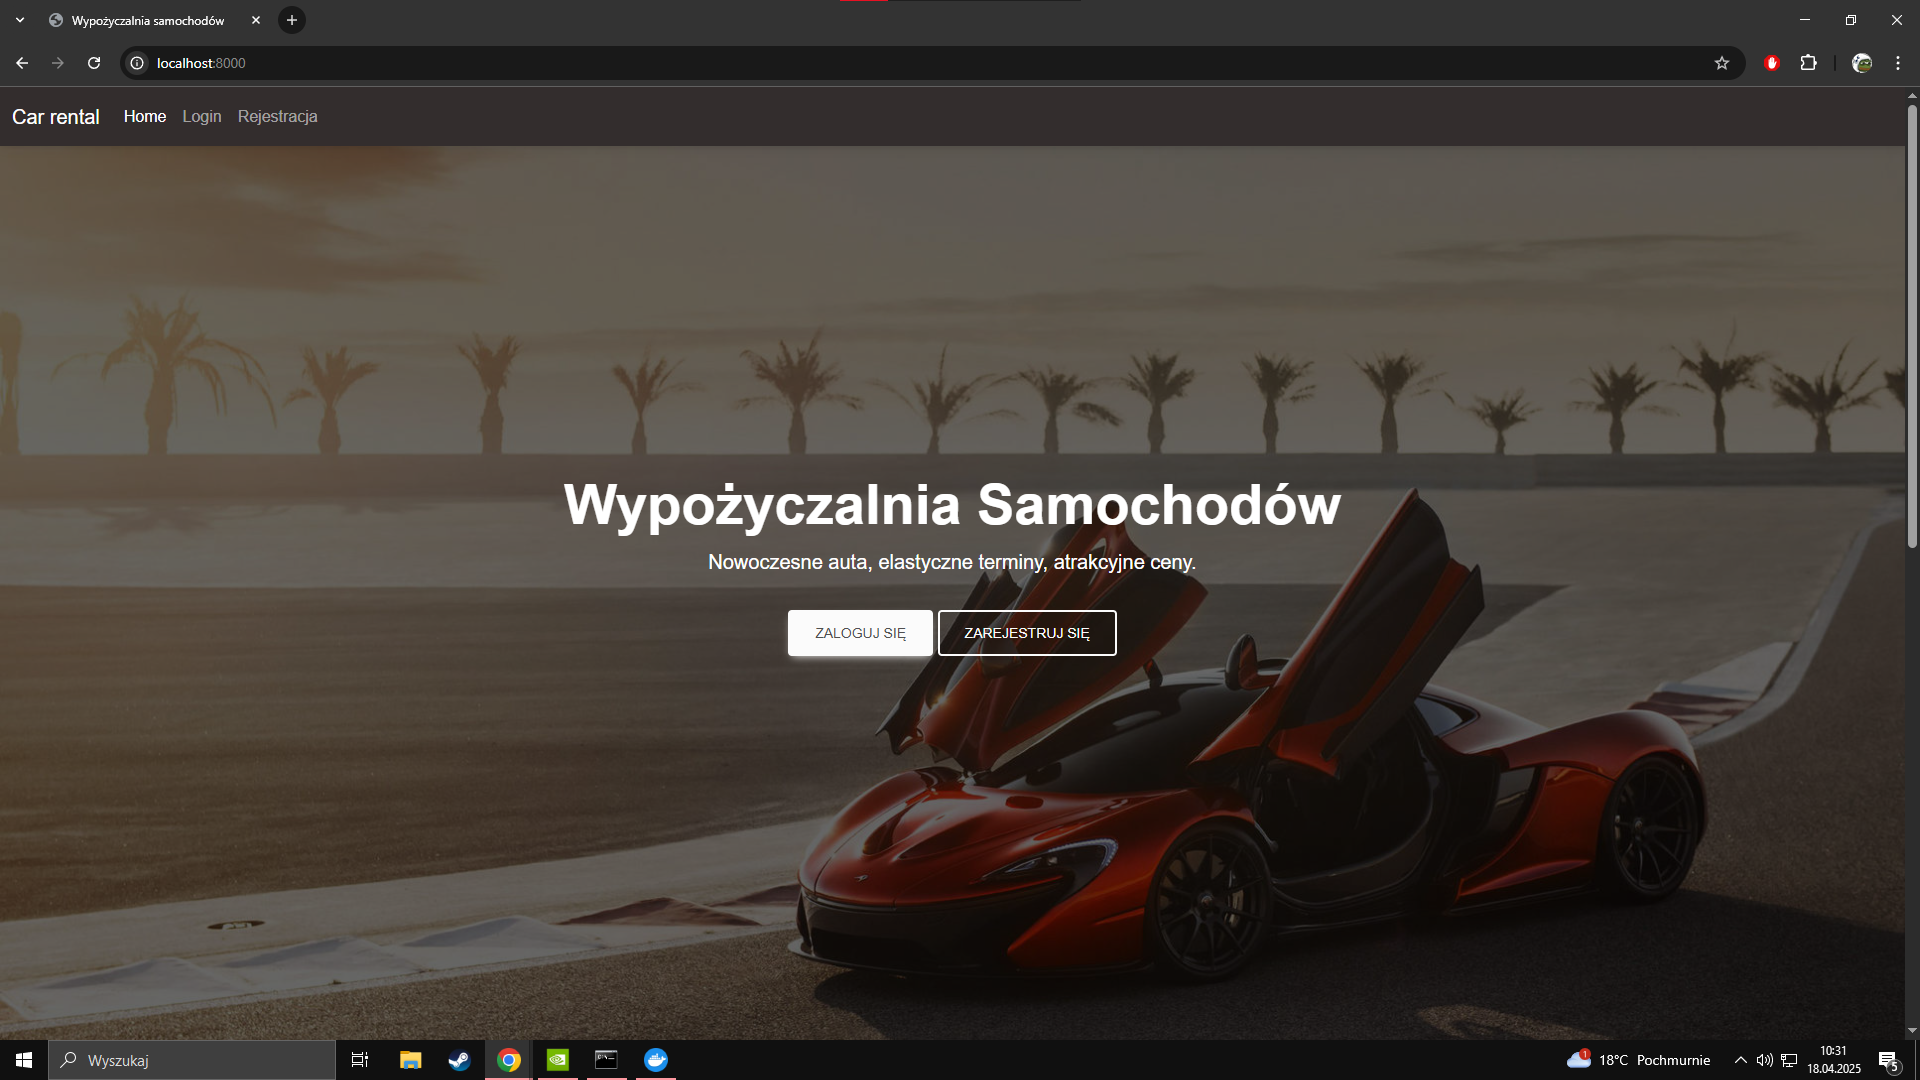
\includegraphics[width=1.1\textwidth]{public_panel.png}
    \caption{Widok strony głównej}
    \label{fig:user-panel}
\end{figure}

\subsubsection{Panel użytkownika}
Dostępny dla zalogowanych klientów:

\begin{enumerate}
    \item \textbf{Strona główna panelu użytkownika (user\_dashboard.html)}
    \begin{itemize}
        \item Wyświetla listę aktualnie dostępnych samochodów wraz z podstawowymi informacjami
        \item Zawiera filtry pozwalające zawęzić wybór samochodów (np. marka, model, rocznik)
        \item Menu nawigacyjne z opcjami: Strona główna, Moje wypożyczenia, Mój profil, Wyloguj
    \end{itemize}
    
    \item \textbf{Strona szczegółów samochodu (car\_detail.html)}
    \begin{itemize}
        \item Prezentuje szczegółowe informacje o wybranym samochodzie
        \item Wyświetla galerię zdjęć z możliwością powiększenia
        \item Zawiera sekcje: specyfikacja, osiągi, opis
        \item Pokazuje dostępność samochodu w kalendarzu
        \item Zawiera przycisk "Wypożycz" prowadzący do formularza wypożyczenia
    \end{itemize}
    
    \item \textbf{Formularz wypożyczenia samochodu (rent\_car.html)}
    \begin{itemize}
        \item Pozwala na wybór daty rozpoczęcia i zakończenia wypożyczenia
        \item Wyświetla koszt wypożyczenia
        \item Zawiera przycisk potwierdzenia wypożyczenia
        \item Waliduje dostępność samochodu w wybranym terminie
        \item Sprawdza, czy użytkownik nie jest na czarnej liście
    \end{itemize}
    
    \item \textbf{Strona moich wypożyczeń}
    \begin{itemize}
        \item Wyświetla listę aktualnych i historycznych wypożyczeń użytkownika
        \item Pokazuje status każdego wypożyczenia (aktywne, zakończone)
        \item Umożliwia podgląd szczegółów każdego wypożyczenia
    \end{itemize}
    
    \item \textbf{Strona mojego profilu}
    \begin{itemize}
        \item Wyświetla dane osobowe użytkownika
        \item Umożliwia edycję danych kontaktowych i adresowych
        \item Pozwala na zmianę hasła
    \end{itemize}
    
    \item \textbf{Strona informacji o blokadzie (user\_ban\_info.html)}
    \begin{itemize}
        \item Wyświetlana, gdy użytkownik jest na czarnej liście
        \item Informuje o powodzie blokady
        \item Pokazuje datę rozpoczęcia i zakończenia blokady
        \item Zawiera informacje kontaktowe do administracji
    \end{itemize}
\end{enumerate}

\begin{figure}[H]
    \centering
    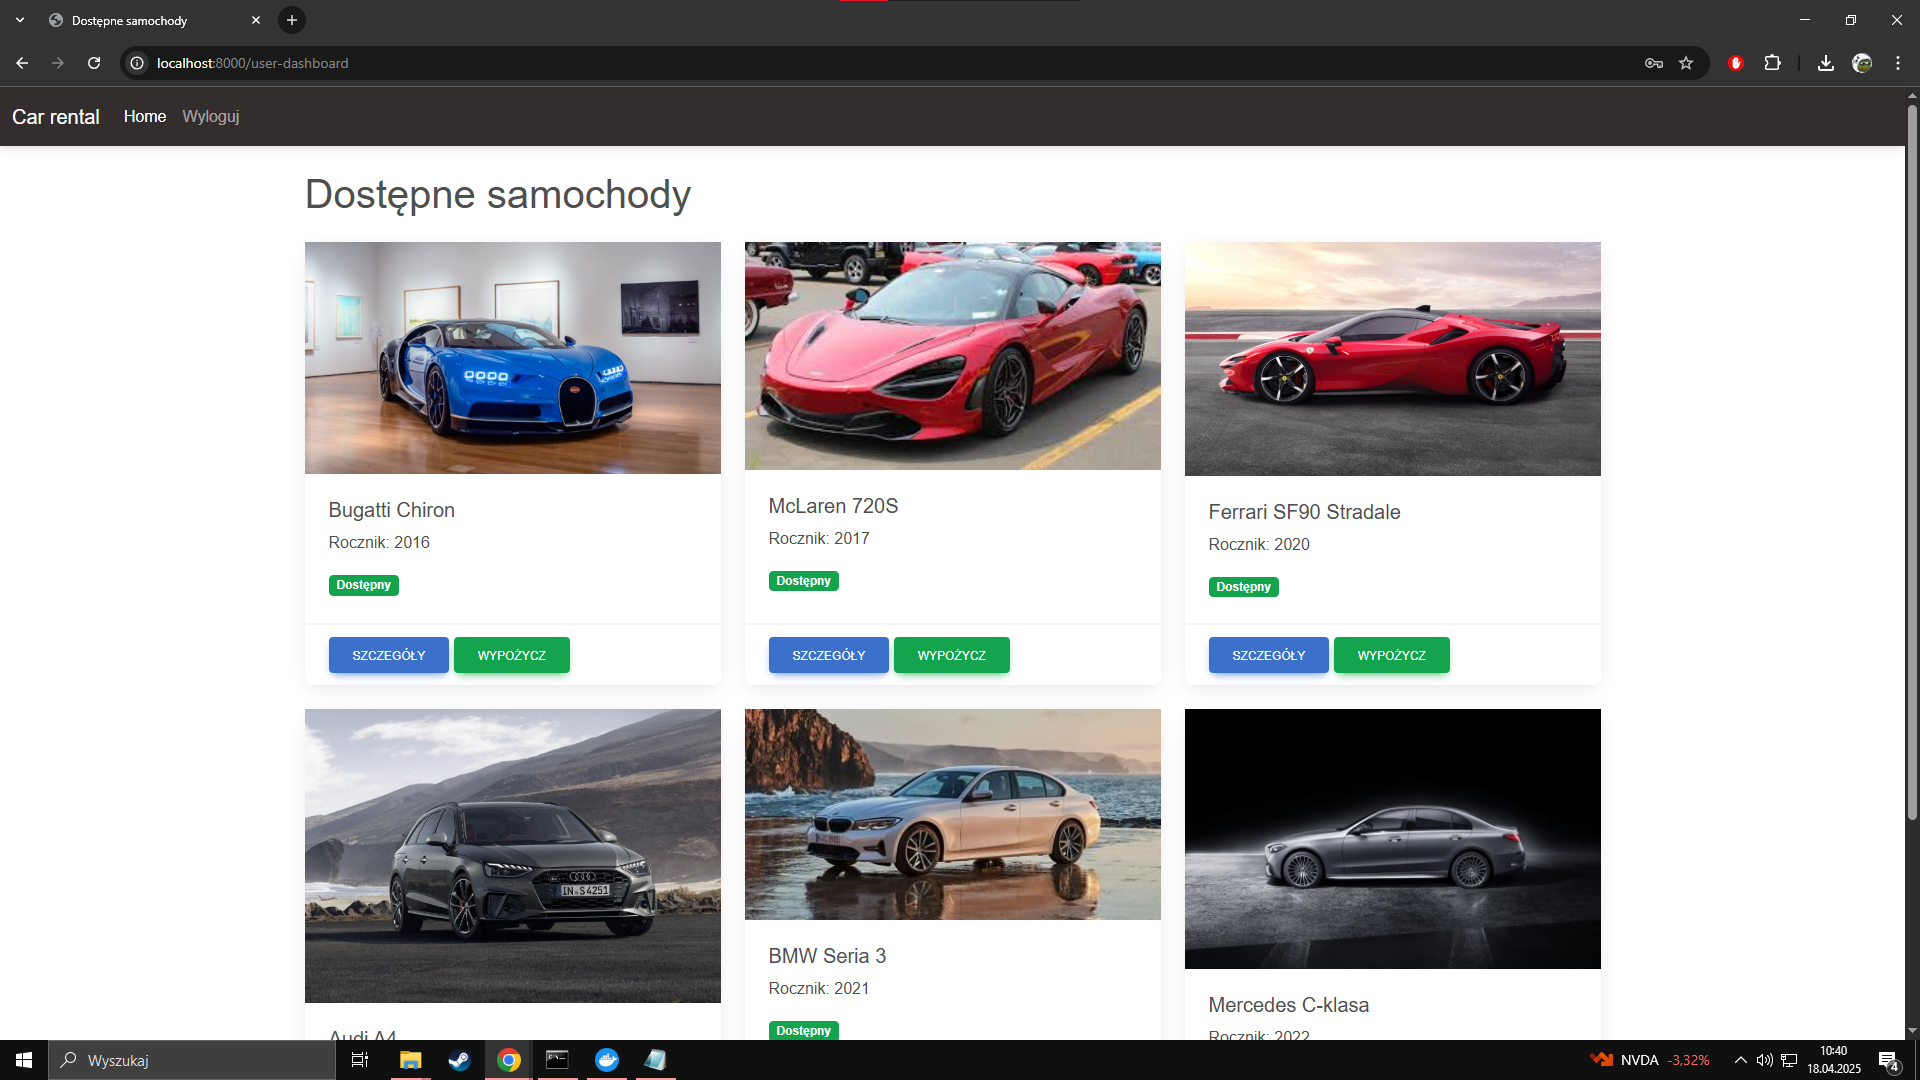
\includegraphics[width=1\textwidth]{user_panel.png}
    \caption{Przykładowy widok panelu użytkownika}
    \label{fig:user-panel}
\end{figure}

\subsubsection{Panel administracyjny}
Dostępny dla zalogowanych administratorów:

\begin{enumerate}
    \item \textbf{Strona główna panelu administratora (admin\_dashboard.html)}
    \begin{itemize}
        \item Wyświetla podsumowanie systemu (liczba samochodów, użytkowników, aktywnych wypożyczeń)
        \item Zawiera skróty do najczęściej używanych funkcji
        \item Menu boczne (sidebar) z dostępem do wszystkich sekcji administracyjnych
        \item Wyświetla alerty o terminach zwrotu samochodów i wygasających blokadach
    \end{itemize}
    
    \item \textbf{Zarządzanie samochodami (admin\_car\_view.html)}
    \begin{itemize}
        \item Lista wszystkich samochodów w systemie z możliwością filtrowania i sortowania
        \item Formularz dodawania nowego samochodu
        \item Opcje edycji i usuwania istniejących samochodów
        \item Przycisk przekierowujący do zarządzania zdjęciami dla wybranego samochodu
    \end{itemize}
    
    \item \textbf{Zarządzanie zdjęciami samochodów (admin\_car\_photos.html)}
    \begin{itemize}
        \item Możliwość dodawania, usuwania i zmiany kolejności zdjęć dla wybranego samochodu
        \item Podgląd wszystkich zdjęć samochodu
        \item Formularz uploadu nowych zdjęć
        \item Drag\&drop do zmiany kolejności zdjęć
    \end{itemize}
    
    \item \textbf{Zarządzanie wypożyczeniami (admin\_rent\_view.html)}
    \begin{itemize}
        \item Lista wszystkich wypożyczeń z możliwością filtrowania (aktywne, zakończone, według dat)
        \item Szczegóły każdego wypożyczenia
        \item Możliwość dodawania, edycji i usuwania wypożyczeń
        \item Oznaczanie wypożyczeń jako zakończone
    \end{itemize}
    
    \item \textbf{Zarządzanie użytkownikami (admin\_user\_view.html)}
    \begin{itemize}
        \item Lista wszystkich użytkowników systemu
        \item Szczegóły każdego użytkownika wraz z historią wypożyczeń
        \item Możliwość dodawania, edycji i usuwania użytkowników
        \item Przycisk do dodawania użytkownika na czarną listę
    \end{itemize}
    
    \item \textbf{Zarządzanie czarną listą (admin\_blacklist\_view.html)}
    \begin{itemize}
        \item Lista użytkowników znajdujących się na czarnej liście
        \item Formularze dodawania użytkowników do czarnej listy
        \item Możliwość edycji powodu i okresu blokady
        \item Opcja usunięcia użytkownika z czarnej listy
    \end{itemize}
    
    \item \textbf{Zarządzanie adresami (admin\_address\_view.html)}
    \begin{itemize}
        \item Lista wszystkich adresów w systemie
        \item Możliwość dodawania, edycji i usuwania adresów
        \item Powiązanie adresów z użytkownikami
    \end{itemize}
    
    \item \textbf{Zarządzanie administratorami (admin\_admin\_view.html)}
    \begin{itemize}
        \item Lista wszystkich administratorów systemu
        \item Możliwość dodawania nowych administratorów
        \item Opcje edycji danych i usuwania administratorów
        \item Zmiana hasła dla administratorów
    \end{itemize}
\end{enumerate}


\begin{figure}[H]
    \centering
    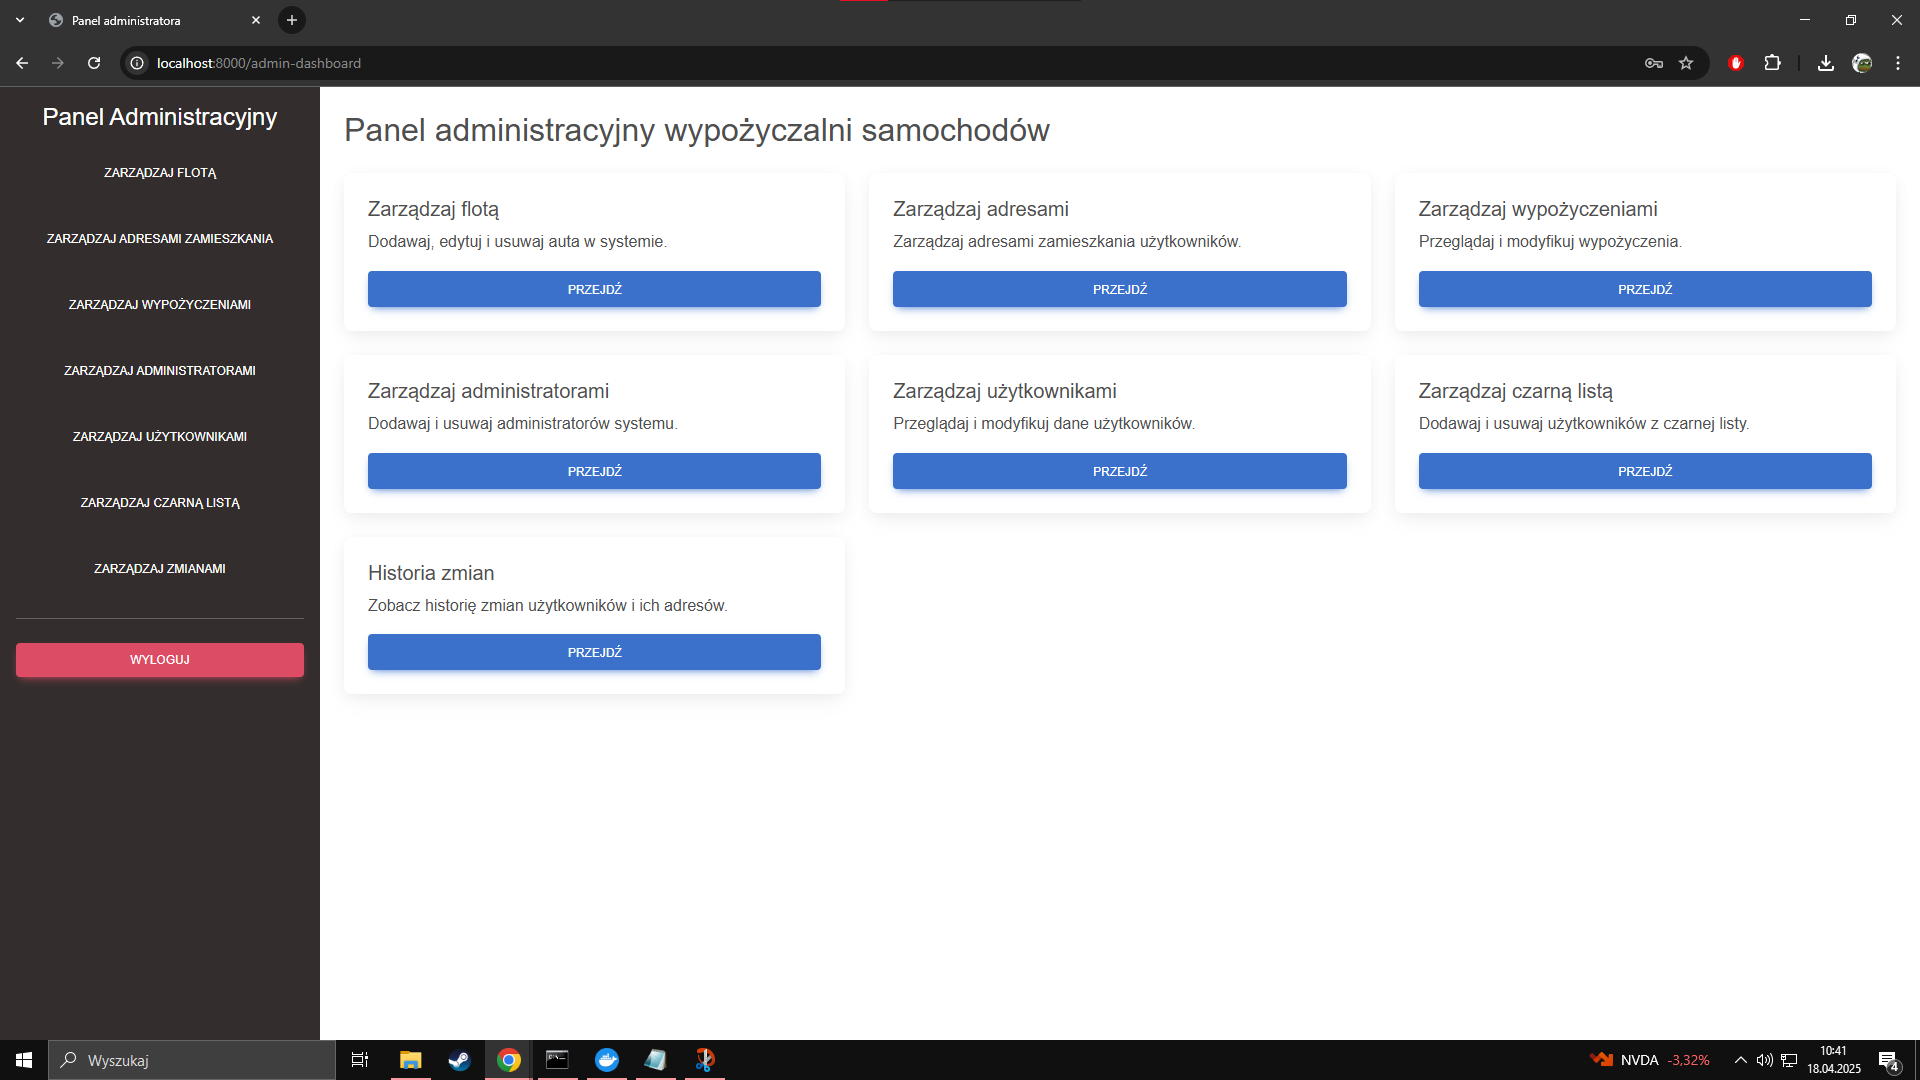
\includegraphics[width=1.1\textwidth]{admin_panel.png}
    \caption{Przykładowy widok panelu administratora}
    \label{fig:admin-panel}
\end{figure}

\newpage

\subsection{Implementacja}

W tej sekcji przedstawiono wybrane fragmenty kodu źródłowego aplikacji, które ilustrują kluczowe aspekty implementacji systemu wypożyczalni samochodów.

\subsubsection{Definicje modeli}

Poniżej przedstawiono przykładową definicję modelu odpowiadającemu tabeli w bazie danych.

\begin{lstlisting}[language=Python, caption={Definicja modelu Auto}]
class Auto(models.Model):
    id_auta = models.AutoField(primary_key=True)
    marka = models.CharField(max_length=100)
    model = models.CharField(max_length=100)
    rocznik = models.IntegerField()
    opis = models.CharField(max_length=1000)
    osiagi = models.CharField(max_length=1000)
    
    def __str__(self):
        return f"{self.marka} {self.model} ({self.rocznik})"
        
    class Meta:
        db_table = 'Auta'
\end{lstlisting}

\subsubsection{Repozytoria danych}

Repozytoria zapewniają warstwę abstrakcji dla operacji na bazie danych, ukrywając bezpośrednie zapytania. Poniżej przedstawiono przykładpwe repozytorium.

\begin{lstlisting}[language=Python, caption={Fragment klasy CarRepository}]
class CarRepository:
    @staticmethod
    def get_all_cars():
        return Auto.objects.all()
    
    @staticmethod
    def get_car_by_id(car_id):
        try:
            return Auto.objects.get(id_auta=car_id)
        except Auto.DoesNotExist:
            return None
    
    @staticmethod
    def get_car_photos(car_id):
        return AutaZdj.objects.filter(id_auta=car_id).order_by('kolejnosc')
\end{lstlisting}

\newpage

\subsubsection{Serwisy biznesowe}

Serwisy implementują logikę biznesową aplikacji, niezależną od warstwy prezentacji.

\begin{lstlisting}[language=Python, caption={Fragment klasy RentalService}]
class RentalService:
    def __init__(self, rental_repository, car_repository, blacklist_repository):
        self.rental_repository = rental_repository
        self.car_repository = car_repository
        self.blacklist_repository = blacklist_repository
    
    def rent_car(self, user_id, car_id, start_date, end_date):
        if self.blacklist_repository.is_user_blacklisted(user_id):
            return False, "Nie możesz wypożyczyć samochodu, ponieważ jesteś na czarnej liście."

        car = self.car_repository.get_car_by_id(car_id)
        if not car:
            return False, "Wybrany samochód nie istnieje."

        if not self.is_car_available(car_id, start_date, end_date):
            return False, "Samochód jest niedostępny w wybranym terminie."
            
        try:
            self.rental_repository.create_rental(user_id, car_id, start_date, end_date)
            return True, "Samochód został pomyślnie wypożyczony."
        except Exception as e:
            return False, f"Wystąpił błąd podczas wypożyczania: {str(e)}"
    
    def is_car_available(self, car_id, start_date, end_date):
        rentals = self.rental_repository.get_car_rentals_in_period(car_id, start_date, end_date)
        return len(rentals) == 0
\end{lstlisting}

\subsubsection{Widoki (Controllers)}

Widoki obsługują żądania HTTP i delegują operacje do odpowiednich serwisów.

\begin{lstlisting}[language=Python, caption={Fragment widoku wypożyczania samochodu}]
@login_required
def rent_car_view(request, car_id):
    car_repository = CarRepository()
    rental_repository = RentalRepository()
    blacklist_repository = BlacklistRepository()
    rental_service = RentalService(rental_repository, car_repository, blacklist_repository)
    
    car = car_repository.get_car_by_id(car_id)
    if not car:
        messages.error(request, "Wybrany samochód nie istnieje.")
        return redirect('user_dashboard')
    
    if request.method == 'POST':
        form = RentCarForm(request.POST)
        if form.is_valid():
            start_date = form.cleaned_data['start_date']
            end_date = form.cleaned_data['end_date']
            
            if start_date < date.today():
                messages.error(request, "Data rozpoczęcia nie może być w przeszłości.")
                return render(request, 'rent_car.html', {'form': form, 'car': car})
            
            if end_date < start_date:
                messages.error(request, "Data zakończenia nie może być wcześniejsza niż data rozpoczęcia.")
                return render(request, 'rent_car.html', {'form': form, 'car': car})

            success, message = rental_service.rent_car(
                request.user.id_user, 
                car_id, 
                start_date, 
                end_date
            )
            
            if success:
                messages.success(request, message)
                return redirect('user_rentals')
            else:
                messages.error(request, message)
                
        else:
            for field, errors in form.errors.items():
                for error in errors:
                    messages.error(request, f"{field}: {error}")
    else:
        form = RentCarForm()
    
    return render(request, 'rent_car.html', {
        'form': form, 
        'car': car
    })
\end{lstlisting}

\subsubsection{Konfiguracja URL}

Plik urls.py definiuje mapowanie adresów URL na funkcje widoków.

\begin{lstlisting}[language=Python, caption={Fragment konfiguracji URL}]
urlpatterns = [
    path('', views.index, name='index'),
    path('login/', views.login_view, name='login'),
    path('register/', views.register_view, name='register'),
    path('logout/', views.logout_view, name='logout'),
    
    path('dashboard/', login_required(views.user_dashboard), name='user_dashboard'),
    path('car/<int:car_id>/', login_required(views.car_detail), name='car_detail'),
    path('rent/<int:car_id>/', login_required(views.rent_car_view), name='rent_car'),
    path('my-rentals/', login_required(views.user_rentals), name='user_rentals'),
    path('profile/', login_required(views.user_profile), name='user_profile'),
    
    path('admin/dashboard/', views.admin_required(views.admin_dashboard), name='admin_dashboard'),
    path('admin/cars/', views.admin_required(views.admin_car_view), name='admin_car_view'),
    path('admin/car-photos/<int:car_id>/', views.admin_required(views.admin_car_photos), name='admin_car_photos'),
    path('admin/rentals/', views.admin_required(views.admin_rent_view), name='admin_rent_view'),
    path('admin/users/', views.admin_required(views.admin_user_view), name='admin_user_view'),
    path('admin/blacklist/', views.admin_required(views.admin_blacklist_view), name='admin_blacklist_view'),
    path('admin/addresses/', views.admin_required(views.admin_address_view), name='admin_address_view'),
    path('admin/admins/', views.admin_required(views.admin_admin_view), name='admin_admin_view'),
    path('admin/history-change/', views.admin_required(views.admin_histroy_change_list), name='admin_history_change_list'),
]
\end{lstlisting}

\newpage

\subsubsection{Walidacja i bezpieczeństwo}

System zawiera mechanizmy walidacji danych oraz zabezpieczenia przed nieautoryzowanym dostępem.

\begin{lstlisting}[language=Python, caption={Dekorator weryfikujący uprawnienia administratora}]
def admin_required(view_func):
    @wraps(view_func)
    def _wrapped_view(request, *args, **kwargs):
        if not request.user.is_authenticated:
            return redirect('login')

        try:
            admin = Admin.objects.get(email=request.user.email)
            request.user.is_admin = True
            return view_func(request, *args, **kwargs)
        except Admin.DoesNotExist:
            messages.error(request, "Nie masz uprawnień do dostępu do panelu administracyjnego.")
            return redirect('index')
    
    return _wrapped_view
\end{lstlisting}

\begin{lstlisting}[language=Python, caption={Walidacja danych formularza}]
class RentCarForm(forms.Form):
    start_date = forms.DateField(
        label="Data rozpoczęcia",
        widget=forms.DateInput(attrs={'type': 'date', 'class': 'form-control'}),
        validators=[MinValueValidator(date.today())]
    )
    end_date = forms.DateField(
        label="Data zakończenia",
        widget=forms.DateInput(attrs={'type': 'date', 'class': 'form-control'})
    )
    
    def clean(self):
        cleaned_data = super().clean()
        start_date = cleaned_data.get('start_date')
        end_date = cleaned_data.get('end_date')
        
        if start_date and end_date:
            if end_date < start_date:
                raise ValidationError(
                    "Data zakończenia nie może być wcześniejsza niż data rozpoczęcia."
                )
            
            if (end_date - start_date).days > 30:
                raise ValidationError(
                    "Maksymalny okres wypożyczenia to 30 dni."
                )
        
        return cleaned_data
\end{lstlisting}

\newpage

\section{Słownik pojęć}

\begin{description}[leftmargin=3.5cm, style=sameline, labelwidth=3cm]
    \item[F] Wymaganie Funkcjonalne (Functional Requirement) - określa funkcję, którą system powinien wykonywać. Opisuje, co system ma robić.
    
    \item[NF] Wymaganie Niefunkcjonalne (Non-Functional Requirement) - określa ograniczenia i cechy jakościowe systemu, takie jak wydajność, bezpieczeństwo, niezawodność czy użyteczność.

    \item[MTV] Model-Template-View - implementacja wzorca MVC w Django, gdzie Model odpowiada za dane, Template (szablon) za prezentację, a View (widok) za logikę biznesową.
    
    \item[Django] Framework webowy napisany w języku Python, wspierający szybkie tworzenie bezpiecznych i skalowalnych aplikacji webowych.
    
    \item[PostgreSQL] Obiektowo-relacyjny system zarządzania bazą danych, wykorzystywany w projekcie jako główne repozytorium danych.
    
    \item[CRUD] Create, Read, Update, Delete - cztery podstawowe operacje trwałego przechowywania danych, odpowiadające za tworzenie, odczytywanie, aktualizowanie i usuwanie rekordów.
    
    \item[Docker] Platforma do konteneryzacji aplikacji, umożliwiająca pakowanie aplikacji wraz z jej zależnościami w standaryzowany sposób.
\end{description}

\end{document}